\documentclass[../main.tex]{subfiles}
\usepackage[utf8]{inputenc}
\usepackage{blindtext}
\usepackage{float}
\usepackage{graphicx}
\usepackage{siunitx}

\begin{document}

This section aims to discuss the current hardware architecture for software-defined satellites (SDS) and how it differs from traditional space information systems, traditional satellites. The pros and cons of such a design choice as well as the current offerings. The differences between SDS as well as traditional satellites will be highlighted.

\section{Old Systems}
Remember that satellites have some necessary components that are absolutely crucial for operation, these include things like:
\begin{itemize}
    \item On-Board Computers (OBC)
    \item Telemetry, Tracking, and Control (TT\&C, typically provided by radios).
    \item Electrical Power System (EPS)
    \item Attitude Determination and Control Systems (ADCS)
    \item Radios
\end{itemize}
The image below showcases some of these components in an architecture diagram of a satellite:
\begin{figure}[H]
    \centering
    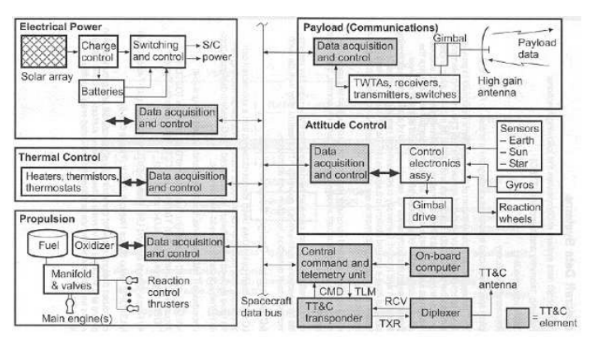
\includegraphics[width=300pt]{images/architecture_satellite.PNG}
    \caption{Satellite Architecture \cite{sat_design}}
    \label{fig:satellite}
\end{figure}
The radio portion is one of the most important parts of a satellite, it's what allows communication and control between the ground station and the satellite itself. Traditionally, the radio put on a satellite served a single purpose, once that purpose was fulfilled the satellites mission was over, there was no other purpose the satellite could serve.

There are many problems with these fixed radios for satellite communications:
\begin{itemize}
    \item Fixed Design
    \item Complex Hardware
    \item More analog components
\end{itemize}
All of this is not to say that there exists no pro, the pros for traditional radios comes in the form of limited processing which allows for freedom when choosing components such as processors, controllers, and analog-digital converters \cite{sdr_satellite}.


\section{New Systems}
With the advent of the software-defined radios (SDRs), traditional radios have started to slowly disappear. An SDR is a transceiver in which, ideally, all of its operation are handled with versatile and general purpose hardware but whose configuration is under software control, hence the software-defined part \cite{sdr_satellite}.

The concept of the SDR was first introduced in 1995 by Joe Mitola. Mitola lays out the key elements needed for the future of radio architecture (shown below). Joe details the following, multi-band antennas, high programmablility, digital mobile cellular radio (MCR), agile modulators and some more.

\begin{figure}[H]
    \centering
    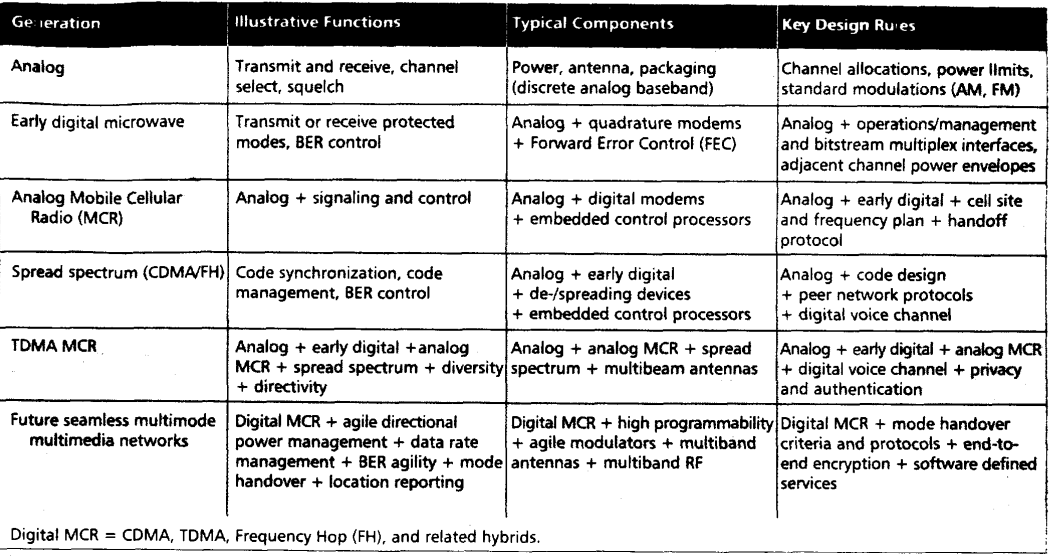
\includegraphics[width=300pt]{images/elements_sdr.PNG}
    \caption{Mitola's Table of Key Elements \cite{sdr_archi}}
    \label{fig:key_elements}
\end{figure}

One of the massive conclusions drawn from Mitola's work was that SDRs should be able to adapt to the air interface by optimizing the carrier frequency, modulation, and choice of radio standard to minimize interference and maintain communication in a given scenario.

\begin{figure}[H]
    \centering
    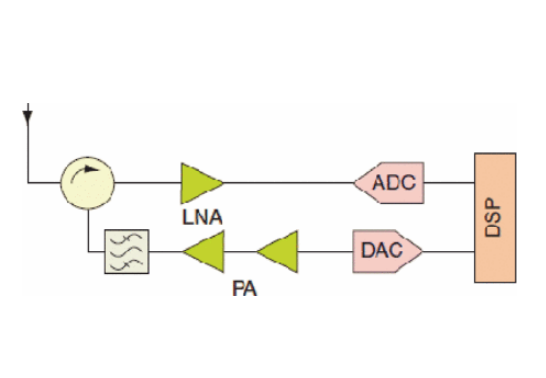
\includegraphics{images/sdr.PNG}
    \caption{Architecture of an ideal SDR \cite{sdr_satellite}\cite{sdr_archi}}
    \label{fig:sdr_architecture}
\end{figure}

The figure above details the steps taken from both the receiving and transmitting end. Below walks through the receiving portion of the SDR \cite{sdr_satellite}:

\begin{itemize}
    \item A signal incident is routed to the Low-Noise Amplifier (LNA) via a circulator.
    \item The signal is then digitized via the analog-digital converter (ADC).
    \item Demodulation/decoding occurs at the Digital Signal Processing (DSP)/Field Programmable Gate Array (FPGA).
\end{itemize}

Below details the steps taken at the transmitting end \cite{sdr_satellite}:

\begin{itemize}
    \item Signals are generated at the DSP/FPGA.
    \item Signals are then up-converted via the digital-analog converter (DAC).
    \item The analog waveforms are amplified and run through a band-pass filter.
    \item Signal are sent through the circulator to the Antenna.
\end{itemize}

All of these improvements help satellites in many ways:

\begin{itemize}
    \item Flexible design
    \item Multi-band
    \item Software based reconfigurable platform
    \item Upgradeable during missions
\end{itemize}

All of these improvements allow satellites to remain useful throughout the entirety of its lifecycle. If the satellite finishes a certain mission, the SDR can be reconfigured for another mission. This fact alone greatly improves the satellites efficiency and efficacy. By allowing for multiple missions during it's lifecycle the satellite is being used to it's full potential.



\end{document}